% Source: graduate-coursework/Sp26/CSCE763/Course_Assignments/Project/project_proposal.tex
% Description: Example PPI radar scan with annotated marine targets. Bright returns (white) represent vessels and buoys; {\color{USC_Garnet

\documentclass[border=4pt]{standalone}
\usepackage{amsmath}
\usepackage{amssymb}
\usepackage{graphicx}
\usepackage{tikz}
\usepackage{xcolor}
\usetikzlibrary{positioning, arrows.meta, calc, fit, backgrounds, decorations.pathreplacing}

\definecolor{USC_Garnet}{HTML}{73000A}
\definecolor{USC_Black10}{HTML}{ECECEC}
\definecolor{USC_Black70}{HTML}{5C5C5C}
\definecolor{USC_Congaree}{HTML}{1F414D}

\begin{document}
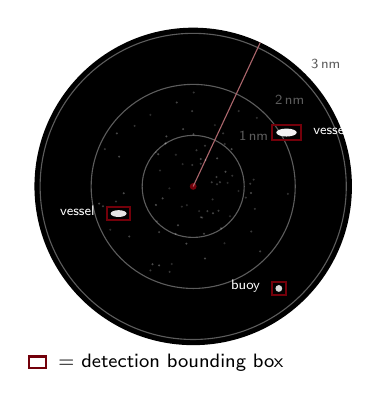
\begin{tikzpicture}[scale=0.72, every node/.style={font=\sffamily\scriptsize}]
  % Background circle (PPI display)
  \fill[black] (0,0) circle (2.8cm);
  % Range rings
  \foreach \r/\lbl in {0.9/1\,nm, 1.8/2\,nm, 2.7/3\,nm} {
    \draw[USC_Black70, thin] (0,0) circle (\r cm);
  }
  % Range ring labels
  \node[USC_Black70, anchor=south west] at (45:0.9cm) {\tiny 1\,nm};
  \node[USC_Black70, anchor=south west] at (45:1.8cm) {\tiny 2\,nm};
  \node[USC_Black70, anchor=south west] at (45:2.7cm) {\tiny 3\,nm};
  % Radar center
  \fill[USC_Garnet] (0,0) circle (0.06cm);
  % Sweep line
  \draw[USC_Garnet!60, thin] (0,0) -- (65:2.8cm);
  % Sea clutter (random dots near center)
  \pgfmathsetseed{42}
  \foreach \i in {1,...,80} {
    \pgfmathparse{rnd*1.4+0.3}\let\cR\pgfmathresult
    \pgfmathparse{rnd*360}\let\cA\pgfmathresult
    \pgfmathparse{rnd*0.15+0.15}\let\cO\pgfmathresult
    \fill[white, opacity=\cO] (\cA:\cR cm) circle (0.02cm);
  }
  % Target 1 — vessel at ~2nm, bearing 30deg
  \fill[white, opacity=0.95] (30:1.9cm) ellipse (0.18cm and 0.07cm);
  \draw[USC_Garnet, thick] ([shift={(-0.25cm,-0.13cm)}]30:1.9cm) rectangle ++(0.5cm,0.26cm);
  % Target 2 — vessel at ~1.5nm, bearing 200deg
  \fill[white, opacity=0.9] (200:1.4cm) ellipse (0.14cm and 0.06cm);
  \draw[USC_Garnet, thick] ([shift={(-0.2cm,-0.11cm)}]200:1.4cm) rectangle ++(0.4cm,0.22cm);
  % Target 3 — buoy at ~2.5nm, bearing 310deg
  \fill[white, opacity=0.85] (310:2.35cm) circle (0.06cm);
  \draw[USC_Garnet, thick] ([shift={(-0.12cm,-0.12cm)}]310:2.35cm) rectangle ++(0.24cm,0.24cm);
  % Labels
  \node[white, anchor=west, font=\sffamily\tiny] at ([shift={(0.3cm,0.05cm)}]30:1.9cm) {vessel};
  \node[white, anchor=east, font=\sffamily\tiny] at ([shift={(-0.25cm,0.05cm)}]200:1.4cm) {vessel};
  \node[white, anchor=east, font=\sffamily\tiny] at ([shift={(-0.16cm,0.05cm)}]310:2.35cm) {buoy};
  % Legend
  \draw[USC_Garnet, thick] (-2.6,-3.2) rectangle +(-0.3,0.2);
  \node[anchor=west, black] at (-2.55,-3.1) {= detection bounding box};
\end{tikzpicture}
\end{document}
